\section{Multilayer perceptrons (MLPs)}

\begin{frame}\frametitle{\secname}

\question{What is a feedforward MLP?} \\

\pause

- A feedforward MLP is a neural network with horizontally stacked vertical columns of connectionist neurons.
\end{frame}

\begin{frame} \frametitle{\secname} 
	\iitem{ layered FFN $y(\cdot; \vec w)$ 
				models label function $y_T(\cdot)$}
	\begin{center} 
		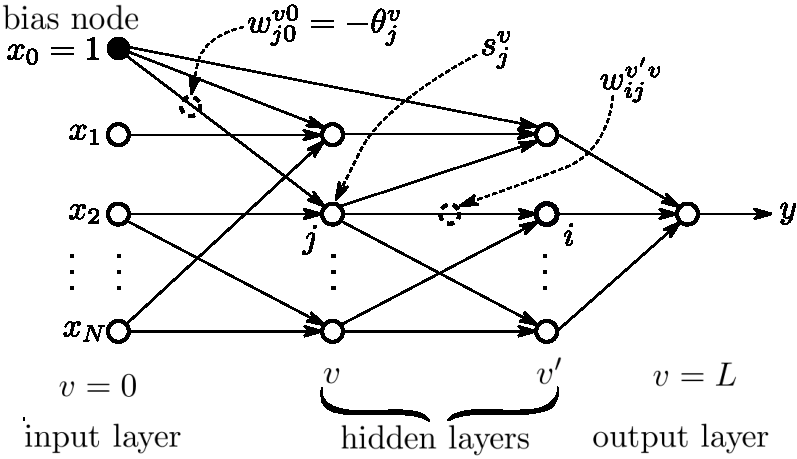
\includegraphics[width=9cm]{img/section1_fig14.pdf} 
	\end{center}
	%\vspace{-4mm}
	\iitem{${\color{blue} s_i^{v'} } = f_i^{v'}( h_i^{v'} ) 
			\stackrel{\text{e.g.}}{=} \tanh(h_i^{v'}) \,, \quad
		h_i^{v'} = \sum\limits_{j=0}^N w_{ij}^{v'v} s_j^v $}
\end{frame}

\subsection{A simple example MLP}

\begin{frame}\frametitle{\subsecname}

1 input, 2 layers
\mode<article>{ (1 hidden layer with 7 nodes + 1 output layer with 1 output node. (i.e. scalar input and scalar output)
}

\begin{figure}[h]
    \centering
		\includegraphics[width=7cm]{img/simpleMLP}
	\caption{Example MLP architecture}
	\label{fig:mlp_example_arch} 
\end{figure}

\only<1>{
\begin{equation}
y({\color{green} x}; \, {\color{blue} \vec W^{10}}, {\color{red} \vec w^{21}}) 
		= { \color{red} f^2_{\,1} \Big(
			{\textstyle\sum\limits_{i=1}^{7}} 
			w^{21}_{1\,i} \; 
			{\color{blue} f_{\,i}^1(w^{10}_{\,i1}\,
				{\color{green}x}-w^{10}_{\,i0}\cdot{\color{green}1})} 
				- w^{21}_{10}\cdot{\color{blue}1}
			\Big) }
\end{equation}

with,
	\begin{equation}
		{\color{blue} f_{\,i}^1(a) = \tanh(a)}
		\;\text{and}\; {\color{red} f_{\,1}^2(a) = a}
	\end{equation}
}
\only<2>{
We can absorb the bias into the weight vector to simplify the notation. 
}
\mode<article>{
We do so by:
}
\end{frame}

\begin{frame}
\mode<presentation>{
\placeimage{8}{0.8}{img/simpleMLP.pdf}{width=5.9cm}	

Simplify notation by:
}
\only<1>{

\begin{enumerate}
\item prepending 1 to the input:\\
	${\color{green} \vec x := (1, x)^\top = (\overbrace{x_0}^{=1}, x_1)^\top}$

\item prepend the bias to each weight vector:\\

$
{\color{blue} 
\vec W^{10} := \rmat{ w^{10}_{10} & w^{10}_{11} \\[1mm] w^{10}_{10} & w^{10}_{11} \\ \vdots\;\, & \vdots\;\, \\ w^{10}_{70} & w^{10}_{71}}
}
\,\text{and}\;
{\color{red} 
\vec w^{21} := \Big(\underbrace{w^{20}_{10}}_{\text{bias}}\,,\, w^{21}_{11}\,,\, \ldots\,,\, w^{21}_{i1}\,,\, \ldots\,,\, w^{21}_{71}\Big)
}
$\\

The first column in ${\color{blue} \vec W^{10}}$ is the bias for each hidden neuron.

\item prepending 1 to the activations in the hidden layer:

\end{enumerate}

Let\\

\begin{align}
{\color{blue} 
\vec{f}^1(\cdot) 
}
:=&
{\color{blue}
\Big(\overbrace{s^1_0}^{=1}\,,\, f^1_1(\cdot) \,,\, \ldots\,,\,, f^1_i(\cdot) \,,\, \ldots\,,\,,f^1_7(\cdot) \Big)^\top
}\\
=&
{\color{blue}
\Big(\,s^1_0\,,\, s^1_1 \,,\, \ldots\,,\,, s^1_i \,,\, \ldots\,,\,,s^1_7\, \Big)^\top = \vec s^1
}
\end{align}

}

\only<2>{

\mode<article>{
From this follows:
}
\mode<presentation>{
\vspace{1cm}
}
\begin{align}
y({\color{green} \vec x}; \, {\color{blue} \vec W^{10}}, {\color{red} \vec w^{21}})
		=&  { \color{red} f^2_{\,1} \Big(
			{\textstyle\sum\limits_{i=1}^{7}} 
			w^{21}_{1\,i} \; 
			{\color{blue} f_{\,i}^1(w^{10}_{\,i1}\,
				{\color{green}x_1}-w^{10}_{\,i0}\cdot{\color{green}x_0})} 
				- w^{21}_{10}\cdot{\color{blue}f^1_0}
			\Big) }\\
		=&  { \color{red} f^2_{\,1} \Big(
			{\textstyle\sum\limits_{i=1}^{7}} 
			w^{21}_{1\,i} \; 
			{\color{blue} f_{\,i}^1({\textstyle\sum\limits_{j=0}^{1}}w^{10}_{\,ij}\,
				{\color{green}x_j})} 
				- w^{21}_{10}\cdot{\color{blue}f^1_0}
			\Big) }\\	
		=&  { \color{red} f^2_{\,1} \Big(
			{\textstyle\sum\limits_{i=1}^{7}} 
			w^{21}_{1\,i} \; 
			{\color{blue} f_{\,i}^1({\vec {W}^{10}} \,
				{\color{green} \vec x})} 
				- w^{21}_{10}\cdot{\color{blue}f^1_0}
			\Big) }\\
		=&  { \color{red} f^2_{\,1} \Big(
			{\vec w^{21}}^{\top} \; 
			{\color{blue} {\vec f}^1({\vec {W}^{10}} \,
				{\color{green} \vec x})}
			\Big) }\\	
		=&  { \color{red} f^2_{\,1} \Big(
			{\vec w^{21}}^{\top} \; 
			{\color{blue} {\vec f}^1(\vec h^1)}
			\Big) } 	\\	
		=&  { \color{red} f^2_{\,1} \Big(
			{\vec w^{21}}^{\top} \; 
			{\color{blue} {\vec s}^1}
			\Big) } 
\end{align}
}

\pause{What are the dimensions for each of the following? \\
${\color{green} \vec x}$, ${\color{blue} \vec W^{10}}$, ${\color{red} \vec w^{21}}$, ${\color{blue} \vec f^1}$, ${\color{red} \vec f^2}$, ${\color{blue} \vec h^1}$}

\pause

\begin{itemize}
\item[--] ${\color{green} \vec x } \in \R^{2,1}$,
\item[--] ${\color{blue} \vec W^{10}}  \in \R^{7,2}$, 
\item[--] ${\color{red} \vec w^{21}} \in \R^{8,1}$, 
\item[--] ${\color{blue} \vec f^1} \in \R^{8,1}$, 
\item[--] ${\color{red} \vec f^2} \in \R$, 
\item[--] ${\color{blue} \vec h^1} \in \R^{\mathbf{7},1}$
\end{itemize}

\end{frame}

\begin{frame}

\question{So what is a deep neural net?}

\pause

- An MLP with many hidden layers and often sparse weight matrices.

\end{frame}
